%=====================================
% PATIENT LEVEL
%=====================================
\chapter{Prise de décision patient}
\label{chap:chapter_6}
\chapterintro
Comme 	
\newpage

\section{Calibration de modèles}
\section{Fusion de décisions}
% Mil & Majority vote\cite{Sudharshan2019}
\section{Approche faiblement supervisée}
\begin{figure}[H]
    \centering
    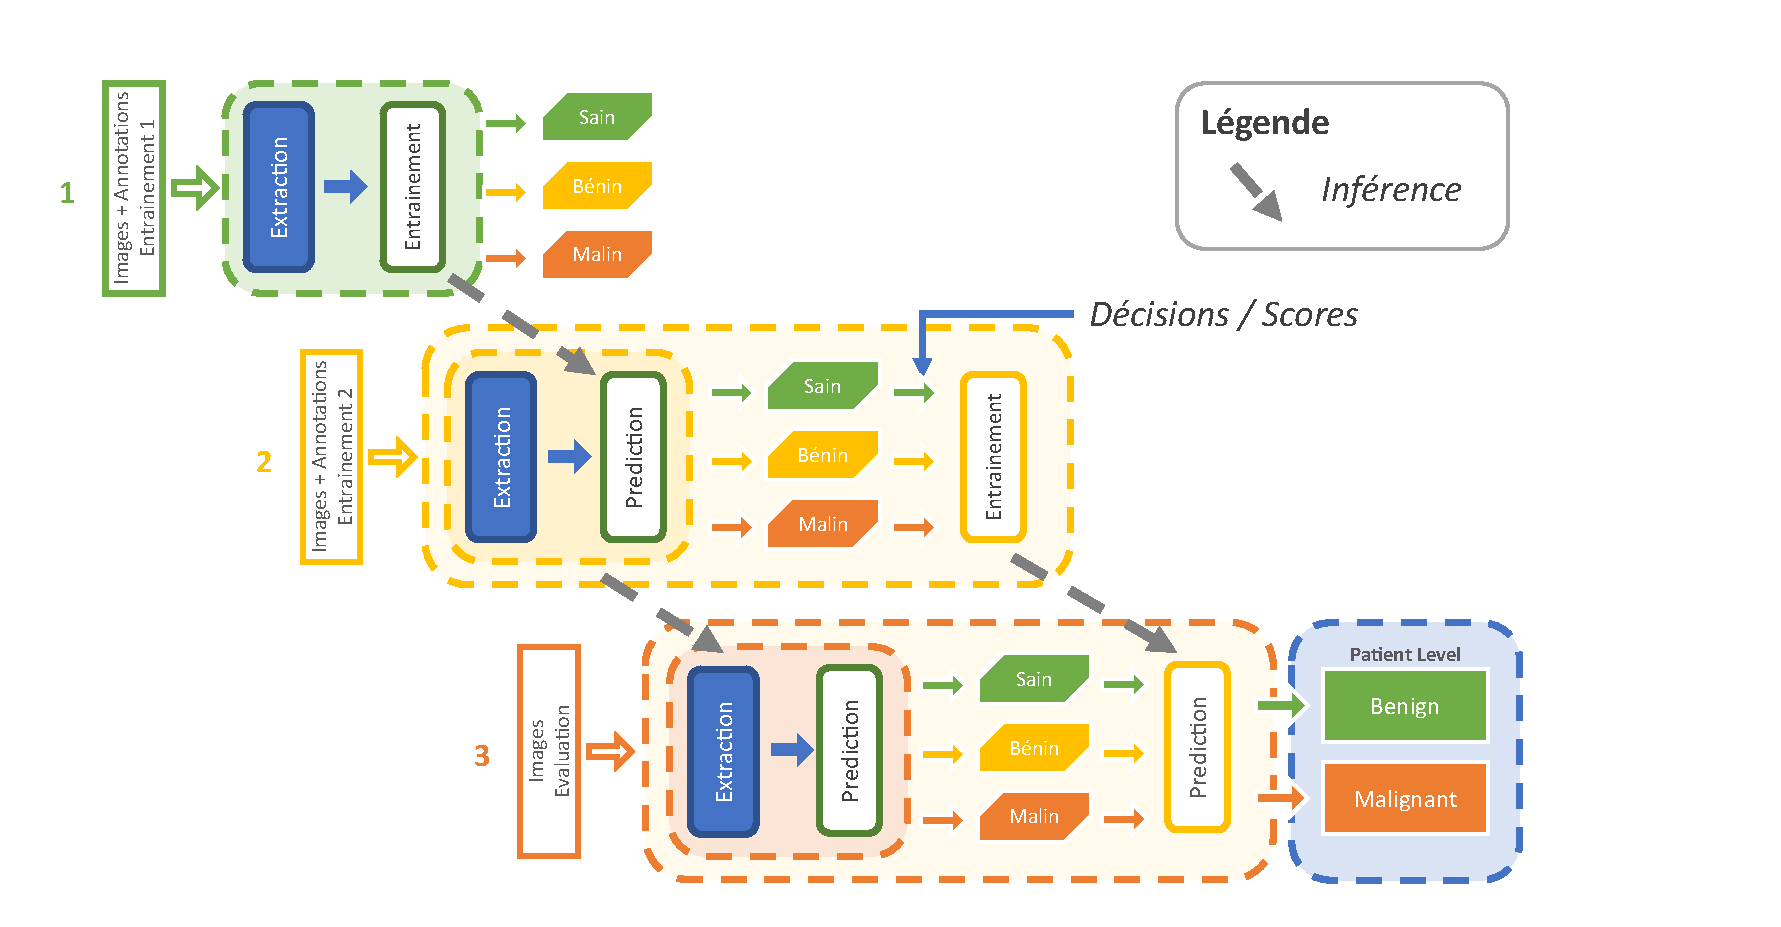
\includegraphics[width=\linewidth]{contents/chapter_6/resources/scheme_patient_decision.pdf}
    \caption{Schéma de représentation du système complet pour la prise de décision patient supervisée.}
    \label{fig:scheme_patient_decision}
\end{figure}\par
\section{Résultat patient}
% This part relates to different ways to achieve classification at the patient-level based on the same two categories: “malignant”, as the positive class, and “benign”. With this assumption, a patient should be considered “malignant” if at least one image is considered to be “malignant”. Additionally, this part needs to consider the varying number of samples per patient (as a reminder, the number of instances per patient can vary between 2 and 833 images).\par
% In order to achieve this, the best combination of the feature extraction method and the classification model from \Cref{sec:image_decision} was used. The classification model provided two types of information for each image: the score was based on prediction probabilities and the decision (i.e., the class that achieved the best probability). In both cases, due to the varying number of images per patient, the information needs to be transformed into constant-size matrices to make a decision for existing and for new patients. At the score level, the structure was composed of patients, images, and scores of classes and transformed into a new matrix of size P*C, where P is the number of patients and C is the number of classes. A dynamic threshold was then used to adjust the positive class that maximizes the chosen metric. Multiple strategies can be used to achieve this:
% \begin{itemize}
% \item Mean - allows the contribution of each instance on the patient to be retained
% \item Maximum – retention of the best confidence prediction as to the trusted one.
% \end{itemize}
% \begin{figure}[H]
%     \begin{center}
%         \includegraphics[width=0.8\linewidth]{Figures/Process_Decision.pdf}
%         \caption{The classification process performed on \ac{rcm} patients in which the first part of the process remained the same as in \Cref{sec:image_decision}. The “Fit Model” and “Prediction” boxes refer to the decision and score level methods discussed in \Cref{sec:patient_decision}. The testing set was predicted for the patients based on “benign” and “malignant” classes.}
%         \label{fig:decision_process}
%     \end{center} 
% \end{figure}\par
% At the decision level, the structure was composed of structure, combining patients, images, and scores of classes and transformed into a new matrix of size P*C, where P is the number of patients and C is the number of classes. Also, C refers to the probability vector of each decision between 0 and 1.
% \begin{itemize}
% \item At Least One - at least one positive decision to consider the input as positive (initial assumption)
% \item Dynamic - find a dynamic threshold that minimizes false-positive decisions.
% \end{itemize}
% A global overview of the processing scheme of this method is presented in \Cref{fig:decision_process}.
% In a second stage, a number of \ac{mil} concepts are implemented in this part, as they fit the issue at hand: a patient is constitutive of several instances (consider it as a bag) and a positive instance assumes that the patient should be positive. Furthermore, only the patient label is known, and the annotation step of individual images is time-consuming. Such a problem can be set as a pair\(\{X|y\}\), in which \(X=\{X^1,X^2,\ldots,X^b\}\) is a bag containing \(b\) instances and each \(X^b\) formulated as follows: \(X^b=\{x^b_1,x^b_2,\ldots,x^b_n\}\), in which \(n\) is the number of features and \(y\) is the patient label~\cite{foulds_frank_2010}. Two ideas are developed regarding this context in the paragraphs that follow. In a first stage, a \ac{sil} classification is used in which a bag is considered as negative if all of the instances are considered to be negative, and positive if at least one of the instances has a positive label that fits our initial formulation of the patient label. In a second stage, the MI-SVM is an extension of \ac{svm} upon \ac{mil} theory and is employed in these due to the results of \Cref{sec:image_decision}. These experiments are configured to function with a linear kernel due to the observation made by the experiments of \Cref{sec:image_decision}. In this part, the experiments were implemented using the “MISVM” library~\cite{Doran2014}.\par
% In addition, to provide the best performance on each of these models, a search for their optimal hyper-parameters was carried out (see \Cref{tab:patient_hyperparameters}).\par
% \begin{table}[H]
%     \centering
%     \begin{tabular}{llll}
%     \textbf{Category}               & \textbf{Name}     & \textbf{Parameter}& \textbf{Values}                                   \\ \hline
%     \multirow{2}{*}{Score}          & Mean              & \multirow{2}{*}{-}& \multirow{2}{*}{[]}                               \\ \cline{2-2}
%                                     & Maximum           &                   &                                                   \\ \hline 
%     \multirow{2}{*}{Decision}       & At Least One      & \multirow{2}{*}{-}& \multirow{2}{*}{[]}                               \\ \cline{2-2}
%                                     & Dynamic           &                   &                                                   \\ \hline 
%     \multirow{2}{*}{\ac{mil}}       & \ac{sil}          & \multirow{2}{*}{C}& \multirow{2}{*}{[0.01, 0.1, 1, 10, 100, 1000]}    \\ \cline{2-2}
%                                     & MI-SVM            &                   &                                                   \\ \hline 
%     \end{tabular}    
%     \caption{List of all of the classification models and referring evaluated hyper-parameters.}
%     \label{tab:patient_hyperparameters}
% \end{table}\par

% The validation protocol remains the same for each of these experiments, based on a nested cross-validation that is known to be less biased than a simple cross-validation scheme~\cite{Cawley2010}. This protocol allows 1) cross-validation of hyper-parameters and 2) objective evaluation of the prediction models. Each of the cross-validation step is based on a K-fold strategy with a $k$ value of 4 on the testing loop and 2 on the validation loop. Also, each time, the patients are separated and balanced as best as possible based on the image labels. In order to achieve an objective evaluation, each data cluster remains the same for the experiments in a given section (refer to \Cref{sec:image_decision} and \Cref{sec:patient_decision}). Moreover, each experiment is validated and evaluated using a \fscore{} metric, as it is statistically suitable for unbalanced populations in comparison with accuracy, and it represents in a single value both recall and precision information. In addition, standard deviation is computed to analyse the stability of models along the nested cross-validation. For this purpose, we used the “Scikit Learn” library for Machine Learning classification, validation, and metric~\cite{pedregosa2011scikit}.\par


% This paragraph focuses on the methods implemented to reach the patient diagnosis (see \Cref{sec:patient_decision}) and it relates to the initial \ac{rcm} data (including unlabeled images) used previously to evaluate specialists~\cite{Cinotti2018}. All these experimental results are listed in \Cref{tab:patient_results} and discussed below. Firstly, the methods performance varied between 0.61 and 0.84 in terms of the \fscore{} for Malignancy. The “At Least One” method achieved poor performance due to prediction errors over the “benign” class. This problem can be solved by the use of a dynamic activation threshold for decisions to minimize the risk of false-positives, at the cost of resulting in an ethical consideration of this method in the clinical context. Secondly, the methods based on the score are almost the same and varied from 0.76 to 0.83 for the \fscore{} for Malignancy. By contrast, with these results, the standard deviations remained reasonable, varying from 0.03 to 0.06. Finally, \ac{mil} was also evaluated, and a substantial difference was noted between the \ac{sil} and the MI-SVM. Indeed, the \ac{sil} assumption yielded similar results with the decision based on the “At Least One” method, due to an insufficient ability to discriminate on the same “benign” class. By contrast, the MI-SVM yielded a number of good results, with an \fscore{} of 0.82. Both methods are stable, with a deviation that only varied from 0.02 to 0.04. Poor results with the “At Least One” and the \ac{sil} methods can be due to a lack of discriminative information provided by the “Inception-ResNet” for these methods.\par
% \begin{table}[H]
%     \centering
%     \begin{tabular}{lllll}
%                                 &                   & \multicolumn{3}{c}{\textbf{Malignancy - \fscore{}}}                    \\ \hline
%     \textbf{Category}           & \textbf{Name}     & \textbf{Weighted}     & \textbf{Benign}       & \textbf{Malignant}    \\ \hline
%     \multirow{2}{*}{Decision}   & At Least One      & 0.61$\pm$0.06         & 0.32$\pm$0.07         & 0.79$\pm$0.05         \\ \cline{2-5} 
%                                 & \textbf{Dynamic}  & \textbf{0.84$\pm$0.03}& \textbf{0.78$\pm$0.07}& \textbf{0.87$\pm$0.02}\\ \hline 
%     \multirow{2}{*}{Score}      & Mean              & 0.83$\pm$0.03         & 0.78$\pm$0.08         & 0.87$\pm$0.02         \\ \cline{2-5}
%                                 & Maximum           & 0.76$\pm$0.04         & 0.68$\pm$0.03         & 0.80$\pm$0.05         \\ \hline  
%     \multirow{2}{*}{\ac{mil}}   & \ac{sil}          & 0.70$\pm$0.04         & 0.50$\pm$0.10         & 0.83$\pm$0.03         \\ \cline{2-5} 
%                                 & \textbf{MI-SVM}   & \textbf{0.82$\pm$0.02}& \textbf{0.78$\pm$0.05}& \textbf{0.84$\pm$0.02}\\ \hline 
%     \end{tabular}    
%     \caption{Results for the patient-level classification for Malignancy (\ac{lm} and \ac{bcc}) according to the different methods from \Cref{sec:patient_decision}. For Malignancy and \ac{lm}, the table provides a weighted average \fscore{} and individual \fscore{} for the benign and the malignant classes.}
%     \label{tab:patient_results}
% \end{table}\par
% Following previous results, this paragraph discusses in detail the results of supervised “Dynamic” decision threshold and \ac{mil} based on “MI-SVM” methods over the Malignancy (meaning \ac{bcc} and \ac{lm}) and \ac{lm} as the cited clinical study does~\cite{Cinotti2018}. \Cref{tab:patient_results_details} provides \fscore{}, precision, and recall based on these experiments. As the classification is binary, recall of the positive class refers to the sensitivity and recall of the negative class refers to the Specificity. The “Dynamic” method achieves scores of 0.89$\pm$0.03 sensitivity and 0.75$\pm$0.07 specificity for Malignancy; 0.88$\pm$0.04 sensitivity and 0.75$\pm$0.07 specificity for \ac{lm} pathologies. The “MI-SVM” method achieves scores of 0.80$\pm$0.02 sensitivity and 0.84$\pm$0.05 specificity for Malignancy; 0.78$\pm$0.07 sensitivity and 0.84$\pm$0.07 specificity for \ac{lm} pathologies. The “Dynamic” method provides more emphasis on sensitivity while “MI-SVM” provides a good specificity. These methods are quite comparable to the evaluation of the dermatologists, reaching 0.80 of sensitivity and 0.81 of specificity, but less homogeneous compared to them.\par
% \par
% \begin{table}[H]
%     \centering
%     \begin{tabular}{lllll||lll}
%                                 &                   & \multicolumn{3}{c}{\textbf{Malignancy}}                               & \multicolumn{3}{c}{\textbf{\ac{lm}}}                                  \\ \hline
%     \textbf{Name}               & \textbf{Label}    & \textbf{\fscore{}}     & \textbf{Precision}    & \textbf{Recall}       & \textbf{\fscore{}}     & \textbf{Precision}    & \textbf{Recall}       \\ \hline
%     \multirow{3}{*}{Dynamic}    & Benign            & 0.78$\pm$0.07         & 0.81$\pm$0.08         & 0.75$\pm$0.07         & 0.79$\pm$0.06         & 0.82$\pm$0.07         & 0.75$\pm$0.07         \\ \cline{2-8}  
%                                 & Malignant         & 0.87$\pm$0.02         & 0.85$\pm$0.03         & 0.89$\pm$0.03         & 0.86$\pm$0.03         & 0.83$\pm$0.03         & 0.88$\pm$0.04         \\ \cline{2-8} 
%                                 & Weighted          & 0.84$\pm$0.03         & 0.84$\pm$0.03         & 0.84$\pm$0.03         & 0.83$\pm$0.03         & 0.83$\pm$0.03         & 0.83$\pm$0.03         \\ \hline
%     \multirow{3}{*}{MI-SVM}     & Benign            & 0.78$\pm$0.02         & 0.72$\pm$0.08         & 0.84$\pm$0.07         & 0.78$\pm$0.05         & 0.73$\pm$0.07         & 0.84$\pm$0.07         \\ \cline{2-8}
%                                 & Malignant         & 0.84$\pm$0.02         & 0.89$\pm$0.05         & 0.80$\pm$0.05         & 0.82$\pm$0.03         & 0.87$\pm$0.06         & 0.78$\pm$0.07         \\ \cline{2-8} 
%                                 & Weighted          & 0.82$\pm$0.02         & 0.82$\pm$0.02         & 0.83$\pm$0.02         & 0.80$\pm$0.03         & 0.80$\pm$0.03         & 0.81$\pm$0.02         \\ \hline 
%     \end{tabular}    
%     \caption{Detailed results for the patient-level classification for the Decision method based on a Dynamic threshold and \ac{mil} based on the MI-SVM assumption. The table provides the \fscore{}, Precision, and Recall for the benign and malignant classes with these methods.}
%     \label{tab:patient_results_details}
% \end{table}\par
% Finally, \Cref{fig:roc_results} provides \ac{roc} curves for both malignancy and \ac{lm} pathologies on “Dynamic” and “MI-SVM” methods. In the context of Malignancy evaluation, the measured \ac{auc} is 0.89 for “MI-SVM” and 0.88 for “Dynamic”. For \ac{lm} evaluation, the measured \ac{auc} is 0.88 for “MI-SVM” and 0.87 for “Dynamic”. In the same context of \ac{lm} lesions, the experts obtained an \ac{auc} score of 0.89, so close to the previous two methods. Apart from this, \Cref{fig:misclassified} provides some misleading images: the \ac{rcm} images in the center belongs to the same patient (image c and d) with similar patterns and homogeneous information while the \ac{rcm} images on the outside parts of the figure contain hair, artifacts, tricky patterns or nonhomogeneous information (image a, b, e, and f). Also, the images on the bottom left and the bottom right (image b and e) of the figure are examples of images were experts will use stacks of images to make their decision and where the currently developed methods only use a single image.
% \begin{figure}[H]
%     \centering
%     \begin{subfigure}{0.47\linewidth}
%         \centering
%         \textbf{Malignancy \ac{roc} curves}\par
%         \includegraphics[width=\linewidth]{Figures/Result_Malignancy.pdf}
%     \end{subfigure}
%     \begin{subfigure}{0.47\linewidth}
%         \centering
%         \textbf{\ac{lm} \ac{roc} curves}\par
%         \includegraphics[width=\linewidth]{Figures/Result_LMM.pdf}
%     \end{subfigure} 
%     \caption{On the left, the \ac{roc} curves for Malignancy with the Dynamic and MI-SVM methods. On the right, the \ac{roc} curves for \ac{lm} with the Dynamic and MI-SVM methods.}
%     \label{fig:roc_results}
% \end{figure}

% \begin{figure}[H]
%     \centering
%     \includegraphics[width=\linewidth]{Figures/Misclassified.pdf}
%     \caption{Examples of \ac{rcm} images that mislead the classifier with the highest \fscore{} (Inception-ResNet + SVM - Linear). On the left part (image a, b and c), \ac{rcm} images belonging to the benign label and classified as malignant. On the right part (image d, e and f), \ac{rcm} images belonging to the malignant label and classified as benign. In the center of the figure (image c and d), two \ac{rcm} images of the same patient belonging to benign and malignant labels.}
%     \label{fig:misclassified}
% \end{figure}